\documentclass[12pt]{article}
\usepackage{multicol}
\usepackage{graphicx}
\usepackage{natbib}
\newcommand{\citeprimsec}[2]{\citep[][cited by \citealp{#2}]{#1}}
\usepackage{amsmath}
\usepackage{amssymb}
\usepackage{mathtools}
\usepackage[english]{babel}
\usepackage{siunitx}
\sisetup{detect-all}
\usepackage[a4paper,width=150mm,top=25mm,bottom=25mm]{geometry}
\numberwithin{equation}{section}

\setlength{\parskip}{\baselineskip}%
\setlength{\parindent}{0pt}%
\begin{document}

\title{Mechanical Engineering: Year One Capstone Assesment}
\date{2019/2020}
\author{University College London}
\maketitle
\begin{flushleft}

\section*{Notes}
\begin{itemize}
  \item Titles are \textbf{not} counted towards the word limit.
  \item References are counted as one word e.g. \citeprimsec{windTurbineMaterial2}{windTurbineMaterial} is counted as \textbf{one} word. This is due to the limitations of \LaTeX \ having no word count feature.
  \item The references section at the end of the document is \textbf{not} counted towards the word limit.
  \item Maths and equations and subsequent words used in equations are \textbf{not} counted towards the word limit e.g. $i = \frac{\omega_{\textrm{output}}}{\omega_{\textrm{input}}}$ the words 'output' and 'input' are not counted here.
  \item The word count for a section is displayed at the end of the last question e.g. the 'Blades' section has five questions and the word count will be displayed after the fifth question.  
\end{itemize}

\section{Blades}
\subsection{For the blades of the wind turbine, composite materials are usually employed. Why is this the case? [74/90 words]}
A composite material may be employed for their favourable properties. Composites materials can have variable (favourable) properties depending on their composition; yielding better fatigue strength, elasticity and corrosion resistance than an alternative e.g. an aluminium alloy. The orientation of the fibres in the composites matrix can be specifically arranged to combat stress (in this case the force of the wind on the blade), reducing the probability of failure (cracking, deformation) in the structure.

\subsection{What common composites might be employed in this application, and what are their relative merits and benefits in comparison to each other? [122/90 words]}
The composite used is likely to be of a fiber-reinforced matrix. The fiber used is likely to be glass or carbon based. Alternatives such as basalt fibers have also been used. Most common are 'E-Glass' fibers, used for their stiffness, tensile and compressive strength. Glass fibers with modified compositions, yielding higher strength, have been developed but are seldom used due to much greater cost.

The matrix material is likely to be a thermoset plastic rather than a thermoplastic. This is due to thermosets having more favourable production characteristics: lower curing temperatures/times and lower viscosity, leading to high processing speed. The most common thermosets used are epoxy and polyester resins. However, an advantage to using a thermoplastic is their recyclability. \citeprimsec{windTurbineMaterial2}{windTurbineMaterial} 

\subsection{What significant issues can you see with using composites in this engineering application? [For 
example, you could consider economic or environmental
challenges] [144/90 words]}
A common manufacturing technique to produce turbine blades is called vacuum assisted resin transfer molding. This is where fiber sheets are placed and aligned in a mold, covered in a vacuum bag and a resin injected. The resin is then left to cure \citep{VARTM}. This process may be labour intensive as the placing and direction of the fibers is a delicate process, requiring human input. Once a blade has been manufactured, the blade must undergo significant testing (in some cases several months), incurring more cost. If a blade is rejected from testing, the material in the blade may be difficult to extract and reuse. 

Building on reuse, recovered fibers prevent a cost barrier as in most cases, recovered fibers are more expensive than new fibers, to use on industrial scales. However, their reuse can be found in other fields, such as cement production \citep{fiberCement}. 

\subsection{The power (W in J/s) produced by a wind turbine depends on blade length (B), the incoming wind speed (V), and air density (\(\rho\)). Derive one dimensionless number relevant to the problem using W as the dependent parameter. Use this dimensionless number to comment on the implications of doubling the blade length. [18/90 words]}
Using Buckingham Pi:
\begin{align}
  [W] &= ML^2T^{-3}\\
  [B] &= L\\
  [V] &= LT^{-1}\\
  [\rho] &= ML^{-3}
\end{align}
\begin{align}
  W &= B^a V^b \rho^c\\
  ML^2T^{-3} &= L^a L^b T^{-b} M^c L^{-3c}\\
  c = 1, b &= 3, a = 2\\
  W &= B^2 V^3 \rho
\end{align}
\begin{gather}
  k = \frac{W_1}{B^2 V^3 \rho} \textrm{ and } k = \frac{W_2}{4B^2 V^3 \rho}\\
  W_1 = \frac{W_2}{4} \\
  4W_1 = W_2
\end{gather}
From this we can see that doubling the blade length (\(B\)), quadruples the power output of the wind turbine.

\subsection{Considering the answer above, discuss the trade-offs associated with choosing longer blades for a turbine of a fixed height. [84/90 words]}
Naturally, choosing larger blades for a turbine of a fixed height creates a limit to how large the blades can be before the turbine’s tower could not structurally support the weight of the blades. Hence, using larger blades requires the use of stronger materials to support their weight. Using stronger materials is more expensive to procure and manufacture, driving up initial costs. If the turbine cannot produce enough power to become economically viable over its lifetime, this would cause problems for the manufacturer.

Words: 442/500

\section{Gearbox (dynamics)}
\subsection{Derive a simple relationship for the gear ratio expressed as a function of number of teeth in the sun and ring gears of an epicyclic (or planetary) gear train.}
Let us define,
\begin{itemize} 
  \item The gear ratio $i$
  \item The sun gear with subscript $S$
  \item The planet gear(s) with subscript $P$ 
  \item The ring gear with subscript $R$
  \item The carrier with subscript $C$
  \item The number of teeth $z$
  \item The modulus of the gear(s) $m$
\end{itemize}

The diameter of a gear is $d = mz$ and for two gears to mesh, their module must be the same. Hence, we can derive
\begin{gather}
  m_1 = m_2\\
  \frac{d_1}{z_1} = \frac{d_2}{z_2}\\
  \frac{z_2}{z_1} = \frac{d_2}{d_1} = \frac{r_2}{r_1}
\end{gather}
From Figure (\ref{SystemRadii}), we can see that a constraint on our system is,
\begin{equation}
  r_R = r_S + 2r_P
  \label{radiiRelationship}
\end{equation}

\begin{figure}[h]
  \centering
  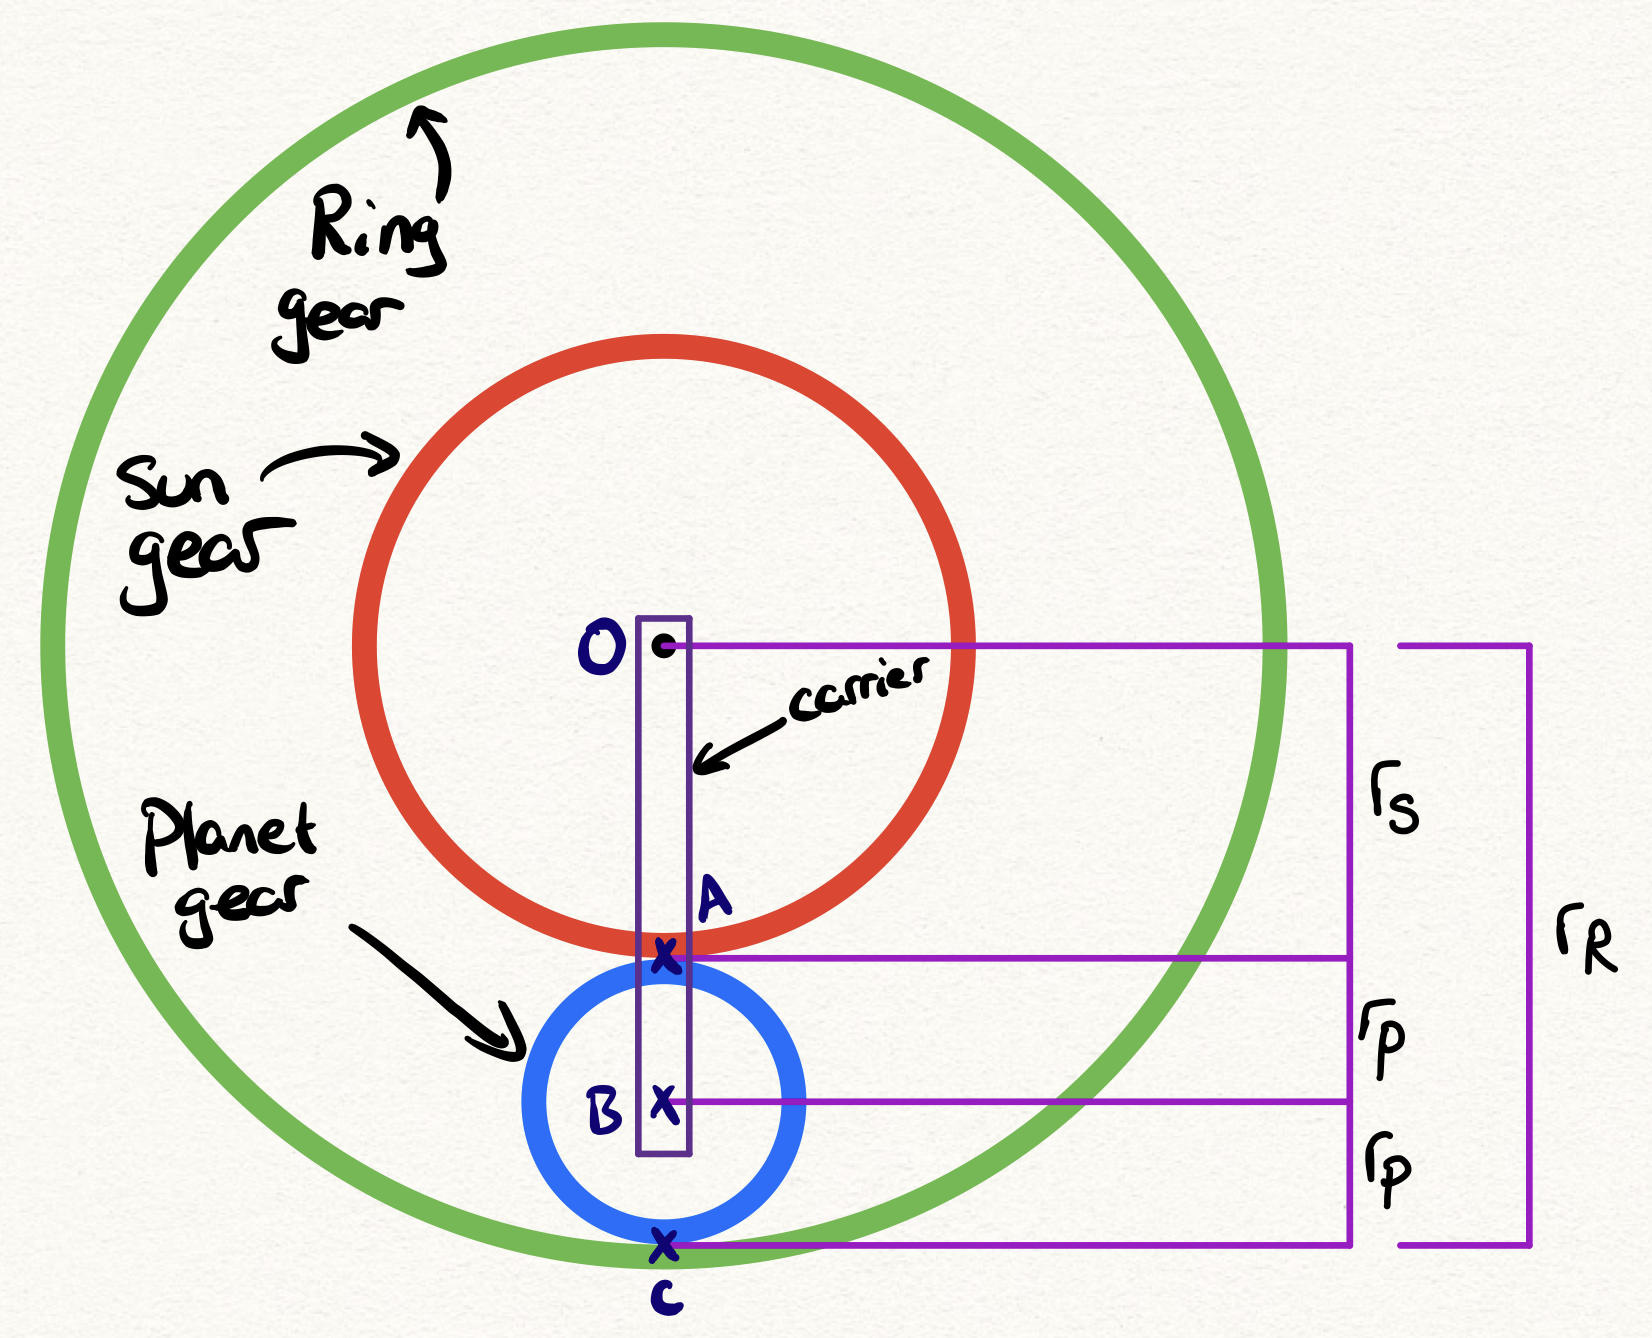
\includegraphics[width = 0.7 \textwidth]{./img/GearRadii.png}
  \caption{Simple planterary gearbox diagram.}
  \label{SystemRadii}
\end{figure}

The gear ratio of a planetary gearbox is given by the following formula.
\begin{equation}
  i = \frac{\omega_{\textrm{output}}}{\omega_{\textrm{input}}}
  \label{gearRatio}
\end{equation}
\subsubsection{Derivation One}
Considering that the sun gear is connected to the input shaft and the carrier of the planet gears is connected to the output shaft, we can simply say,
\begin{equation}
  i = \frac{\omega_S}{\omega_C}
\end{equation}
The linear velocity of the carrier is,
\begin{equation}
  v_C = \omega_C (r_S + r_P)
\end{equation}
The velocity of the point of contact between the sun and the planet gear is,
\begin{equation}
  v_S = \omega_S r_S
\end{equation}
By considering the point of contact between the planet and the ring gear as having 0 relative velocity, we can derive that the point of contact between the sun and the planet is simply $2v_C$. Hence,
\begin{align}
  v_S = 2v_C &= 2\omega_C(r_S + r_P)\\
  \omega_S r_S &= 2\omega_C (r_S + r_P)\\
  \frac{\omega_S}{\omega_C} &= \frac{2(r_S + r_P)}{r_S}\\
  &= \frac{2r_S + 2r_P}{r_S} \label{gearRatio1}
\end{align}
Rearranging equation (\ref{radiiRelationship}) and substituting into (\ref{gearRatio1}), we get,
\begin{align}
  \frac{\omega_S}{\omega_C} &= \frac{2r_S + r_R - r_S}{r_S}\\
  &= \frac{r_S + r_R}{r_S}
\end{align}
This simplifies to,
\begin{equation}
  i = 1 + \frac{r_R}{r_S}
\end{equation}
Since the number of teeth is proportional to the radius of the gear, we can substitute $z$ into our equation,
\begin{equation}
  i = 1 + \frac{z_R}{z_S}
\end{equation}
\subsubsection{Derivation Two (MERT AYDIN DEVELİOĞLU'NUN İZNİYLE)}
Point A experiences fixed axis rotation about centre $0$. Hence,
\begin{equation}
  v_S = \omega_S r_S
  \label{dev2Eq1}
\end{equation}
The velocity at point A can also be written as:
\begin{equation}
  v_S = v_R + v_{S/R}
\end{equation}
In the case where the ring gear is stationary, \(v_R = 0\). Subsituting this we arrive at,
\begin{equation}
  v_S = \omega_P(2r_P)
  \label{dev2Eq2}
\end{equation}
Equating equations (\ref{dev2Eq1}) and (\ref{dev2Eq2}) yields:
\begin{align}
  \omega_S r_S &= \omega_P (2r_P)\\
  \omega_P &= \frac{\omega_S r_S}{2r_P} \label{dev2Eq3}
\end{align}
Point B experience fixed axis rotation about centre $0$. Hence, 
\begin{equation}
  v_C = \omega_C r_C = \omega_C (r_S + r_P) \label{dev2Eq4}
\end{equation}
The velocity at point B can also be written as:
\begin{equation}
  v_C = v_R + v_{C/R} = 0 + r_P \omega_P \label{dev2Eq5}
\end{equation}
Using equations (\ref{dev2Eq3}), (\ref{dev2Eq4}) and (\ref{dev2Eq5}) yields:
\begin{align}
  \omega_C (r_S + r_P) &= r_P \frac{\omega_W r_S}{2r_P}\\
  \frac{\omega_S}{\omega_C} &= \frac{2(r_S + r_P)}{r_S} \label{dev2Eq6}
\end{align}
Using equation (\ref{radiiRelationship}) into (\ref{dev2Eq6}) yields:
\begin{align}
  \frac{\omega_s}{\omega_C} &= \frac{2r_S + r_R - r_S}{r_S}\\
  \frac{\omega_s}{\omega_C} &= \frac{r_S + r_R}{r_S}
\end{align}
Hence, the gear ratio $i$ is:
\begin{equation}
  i = \frac{r_S + r_R}{r_S} = 1 + \frac{r_R}{r_S}
\end{equation}
Since the number of teeth is proportional to the radius of the gear, we can substitute $z$ into our equation,
\begin{equation}
  i = 1 + \frac{z_R}{z_S}
\end{equation}
\subsection{Perform a conceptual design of an epicyclic gear system for a 1.5 MW wind turbine if the three blades spin at a design speed of 12 rpm and the high-speed shaft in the generator needs to spin at 1680 rpm. Provide information on the configuration of your proposed planetary gear set (note: the 5 laws of planetary gearing – see the provided videos) and the input/output torque ratio that can be achieved by your system. Neglect friction and assume that the angular acceleration of the gears (which are rigid and non-deformable) is zero. You must indicate the number of teeth in each gear and provide a schematic drawing.}
\subsection{Wind gusts and turbulence lead to misalignment of the drive train and premature failure of the gear components. How could this be mitigated? [132/150 words]}
Misalignment of the gear teeth can cause parts of the gear to undergo more wear and tear than normal. This could take place when the gears grind together. This abrasive action would cause more particulate matter to be generated when the gearbox is in operation.This will cause further damage as these particles will scratch, cut and gouge more material out of the gears. This can be mitigated with adequate lubrication of the gears, as it will keep the gears clean, cool and prevent a buildup of dirt. 

Prevention of failure can also occur through maintenance inspections of the gearbox. A technician inspecting the gearbox will identify signs of failure in the gears and replace components where needed. Processes such as cleaning can also take place to prevent further failure from occurring.

\subsection{Comment on the advantages/disadvantages of an epicyclic gear system in the context of a wind turbine gear box. [170/150 words]}
Considering that wind turbines are designed to generate power in the MWs, the gearbox must be able to withstand high torque, be small, lightweight and have great design efficiency. In an epicyclic gear system, the input load is shared between multiple planet gears. This makes them ideal for high torque use cases as the force is shared between multiple planets. Epicyclic gear systems are more efficient when compared to traditional gearboxes, as the driving member and the driven member are concentrically aligned. This allows multiple planets to be placed together in a gearbox, allowing for very high gear ratios in a small and compact size.

However, the cost to develop an epicyclic gear system is higher than a traditional gearbox. The design is more complex and because of this; it requires a higher engineering accuracy to develop the components. This design complexity also makes these gearboxes harder to maintain.

To conclude, epicyclic gear systems are a suitable fit for a wind turbine for their design efficiency and high torque capability.

\section{Gearbox (materials)}
\subsection{For the gears in the gearbox of the wind turbine, steel would normally be the material of choice. Why is this the case? [61/150 words]}
Steel is cheap and available in a range of strengths, dependent on the carbon content. It is also tough and ductile. Steel is heat treatable and alloys with many other elements such as Chromium, Manganese and Nickel, changing its properties further. This makes steel (and its alloys) a very versatile material: easily bought and manufactured to suit the task at hand.
\subsection{There are many different grades of steel available – what particular properties of the steel might be required for a gearbox application, and what sorts of steel would be suitable therefore? [301/150 words]}
Let us think about the potential failures which may occur with the gears in the gearbox. Gear teeth can wear and break. Hence, we require steel with good (surface) hardness. As a side note, we may utilise lubrication to reduce the impact of shear forces on the gear. This will also help in keeping dirt and debris away from our gears, preventing misalignment and breakdown. 

The gear will be expected to have excellent longevity. On average, a wind turbine is expected to last twenty years \citep{windTurbineLifetime}. Since the wind is not a constant force, the application of forces on our gears will be cyclic. Thus the steel used should have adequate fatigue strength. The way our gear is designed will also affect this property, e.g. making sure there are no stress concentrations and making sure there is a good surface finish/contact. Manufacturing the gear this way will help reduce the potential for failure points to grow and manifest into fractures. 

We must also consider the operating conditions of our gears. Since our gearbox will be housed in the turbine's nacelle, we can assume that our gearbox will be protected from weather. The gearbox will still undergo temperature changes. Depending on the location of the wind turbine, the gears must be designed to work with the local climate in mind. Wind turbines operating in sub 20\si{\celsius} or plus 50\si{\celsius} temperatures must be designed with special considerations given to the components and infrastructure \citep{windTurbineOperatingConditions}. 

Gears must be manufactured to have certain properties,
\begin{itemize}
  \item High tensile strength - prevention of failure when a torque (static load) is applied to the gear.
  \item High fatigue strength - withstand the dynamic loads when the gear is in use.
  \item Low coefficient of friction - reduce mechanical losses in the system.
  \item Good manufacturability - to reduce cost.
\end{itemize}
\subsection{The gears will be enclosed in a housing to help hold the mechanism together and prevent the ingress of contaminants. Suggest suitable materials for this housing, ensuring you provide justification for your suggestions (taking into account a range of factors including properties, and economic issues). Given your suggestions above, qualify these by providing consideration for how such an enclosure could be manufactured. What manufacturing processes might principally be required?}

\section{Tower}
\subsection{The tower in the picture is a single tube which is also normally made of steel. Explain why this is likely to be manufactured from a different grade of steel to that used in the gearbox. What properties are needed in this particular context? [161/150 words]}
The wind turbine’s tower is expected to be a particular grade of steel because of the forces applied to the material. A factor to consider is how the wind force can induce an oscillation in the tower. The stiffness of the steel and natural frequency of the tower will play a dominant role in diminishing oscillations and avoiding resonance. A stiff steel will be more suitable in this context. 

Considering that the nacelle and blades atop the tower, they exhibit a downward force on the tower, compressing it. Hence, a steel with adequate compressive strength and ultimate stress to support the weight of the turbine is required. This is contrary to the steel used for the gears as they have high tensile strength. 

Our wind turbine will again be subject to a variety of forces over its lifetime. Wind turbines are designed to have long lifespans, hence we can mitigate failure (in the material) using a high fatigue strength steel.  

\section{Energy generation}
\subsection{Designers are considering the maximum power that could be generated by this turbine in two theoretical case studies. In case A, the incoming wind speed is 25 m/s and the air speed after passing through the blades is 15 m/s. In case B, the incoming wind speed is 20 m/s and the final speed is 12 m/s. Describe the concepts needed to estimate the maximum theoretical output of a wind turbine, and calculate the maximum theoretical power output for both these cases when the blade length is 37 m. Take the value of 1.2 kg/m3 for air density.}
\subsubsection{Case A}
Variables:
\begin{itemize}
  \item $V_{in} = 25\si{\meter\per\second}$
  \item $V_{out} = 15\si{\meter\per\second}$
  \item $B = 37\si{\meter}$
  \item $\rho_{air} = 1.2\si{\kg\per\meter\cubed}$
\end{itemize}
Power is given by:
\begin{equation}
  \textrm{Power} = \textrm{Force} \times \textrm{Velocity}
\end{equation}
Hence,
\begin{equation}
  P = \frac{1}{4} \rho A (V_{out} + V_{in})(V_{out}^2 - V_{in}^2)
\end{equation}
\subsubsection{Case B}

\subsection{Consider the various terms in the energy equation as they relate to a wind turbine. Describe briefly which terms are important for the wind turbine, and connect terms in the equation to the major sources of energy loss. Comment on the implications for wind turbine efficiency.}
\subsection{The world’s most powerful commercial wind turbine today has a blade length of 82m and is rated at 9.5 MW. Comment briefly on the reasons why the numbers calculated using your theoretical approach above are far larger than this actual capacity.}

\section{Energy storage}
\subsection{In an offshore wind turbine facility, the excess energy generated is stored using a simple compressed air storage system. The wind turbine is mechanically coupled to a compressor that has a compression ratio of 200. The compressor takes in air from the surrounding at ambient pressure and temperature conditions (p0, T0) and performs a reversible adiabatic compression process. The output air from the compressor (at p1, T1) undergoes a reversible isobaric heat removal process using a heat exchanger in order to reduce the temperature to T0. The air is then stored in a high-pressure storage facility.}
\subsection{Determine:}
\subsubsection{heat and work transfers per unit mass for both the compression and heat removal processes}
\subsubsection{the total entropy change per unit mass undergone by air}
\subsection{The heat removal in the above system is achieved by a refrigerator operating on a simple vapour compression cycle. This simple vapour compression refrigerator uses ammonia (NH3) as the working fluid. The evaporator pressure is pe and the condenser pressure is pc (where pc/pe>=6). The working fluid leaves the evaporator dry-saturated and enters the compressor, where it is compressed reversibly and adiabatically. Condensation at constant pressure then takes place until the saturated liquid state is reached. This is followed by throttling to evaporator pressure.}
\subsection{Sketch the cycle on T-s and p-h diagrams}
\subsubsection{the compressor delivery temperature, and}
\subsubsection{the mass flow rate of the refrigerant}

\section{Final discussion}
\subsection{Consider all the aspects covered above and compare the trade-offs in each of these categories during wind turbine design. You may also wish to consider how they are affected by the environment: water depth, ocean waves and seafloor structure. Reflect on the consequent additional challenges in building and maintaining offshore wind turbines.}
test

\bibliographystyle{agsm}
\bibliography{references}
\end{flushleft}
\end{document}